\documentclass[12pt]{article}

% Language setting
\usepackage[utf8]{inputenc}
\usepackage[bulgarian]{babel}

% --------------------- Packages  --------------------
% Use biblatex
\usepackage{biblatex}
\addbibresource{bibliography.bib}
% Table thickness
\usepackage{ctable}
% Equations: SI units
\usepackage{siunitx}
% Approximately equal
\usepackage{amssymb}
% degrees symbol
\usepackage{gensymb}

% --------------------- Title  --------------------
\addbibresource{bibliography.bib}
\title{Косвено измерване на обем на тяло}
\author{Виолета Кабаджова}
\date{October 2022}

\begin{document}

% Anfang der Titelseite________________________________________________________________________________
\begin{titlepage}
	\flushleft
% 	\begin{center}
	%{\scshape\Large Werkstoffe III \hspace{2.5cm} Laborbericht \hspace{2.5cm}HS 2022 \par}
	{\scshape\Large Протокол I \hspace{2.5cm} Механика - практикум\par}
	\vspace{5cm}
	{\huge\bfseries Косвено измерване на обем на тяло\par}
	\vspace{1cm}
	{\LARGE\bfseries Лабораторно упражнение №1\par}
	\vspace{5cm}
    % {\LARGE\bfseries Физически Факлутет към Софийски Университет ``Св. Климент Охридски \par}
    {\LARGE\bfseries Виолета Кабаджова, \par}
%   {\LARGE\bfseries Group: X\par}
    {\large\bfseries ККТФ, факл. номер: 3PH0600026\par}
	\vspace{1cm}
	
	{\large Физически Факлутет, 
	
	Софийски Университет "Св. Климент Охридски"
	
	20 Октомври 2022 г.\par}
	
\end{titlepage}

\section{Теоритична част}

\subsection{Нониус и микрометричен винт}
Нониусът и микрометричният винт са скали, които ни позволяват да отчетем най-малкото дробно деление на основната скала. Докато нониусът се движи праволинейно по основната си скала, за която е прикрепен, то микрометричният винт превръща въртеливото движение на винта в праволинейно движение по оста на въртене. Точността и на двете се характеризира чрез т.нар. инструментална константа, определяща инструменталната грешка. При правия нониус (\begin{math}a > b\end{math}) тя е равна на:

\begin{displaymath}
k = a - b = a - a\frac{n-1}{n} = \frac{a}{n},
\end{displaymath}

където а - стоийността на най-малкото скално деление, b - стойността на най-малкото деление на нониусовата скала, n - броя на деленията на нониуса. Горната формула следва от факта, че дължината на всички n деления на нониуса е равна на n - 1 деления на основната скала, откъдето следва, че \begin{math} n b=(n-1)a \end{math}. Това е при положение, че нониусът е от вида на т.нар. прави нониуси, при които a > b. Съществуват и т.нар. обратни нониуси, при които стойността на най-малкото скално деление на основната скала a е по-малко от стойността на най-малкото деление на нониусовата скала (\begin{math} a < b \end{math}). Тогава константата \begin{math} k < 0 \end{math} и \begin{math} k = - \frac{a}{n} \end{math}. Нониусовата константа k е равна на инструменталната грешка.

Микрометричният винт от своя страна работи чрез въртеливо движение. При него: 

\begin{displaymath}
k = \frac{h}{n},
\end{displaymath}

където h - стъпка на винта (разстоянието, на което се премества винта по основната скала след завъртане на пълен оборот от 360\degree), n - броя на микрометричните деления. Стойността на най-малкото деление на микрометричната скала, въведено като b при нониуса, е избрана така, че \begin{math}h = nb \end{math}. Полезно е да се отбележи, че при завъртане на винта на ъгъл \begin{math} \alpha \end{math}, преместването ще бъде \begin{math} h_\alpha = \frac{360\degree}{\alpha}\end{math}. Инструменталната грешка на микрометричния винт е равна на половината от микрометричната константа k.

\subsection{Шублер}
\begin{figure}
    \centering
    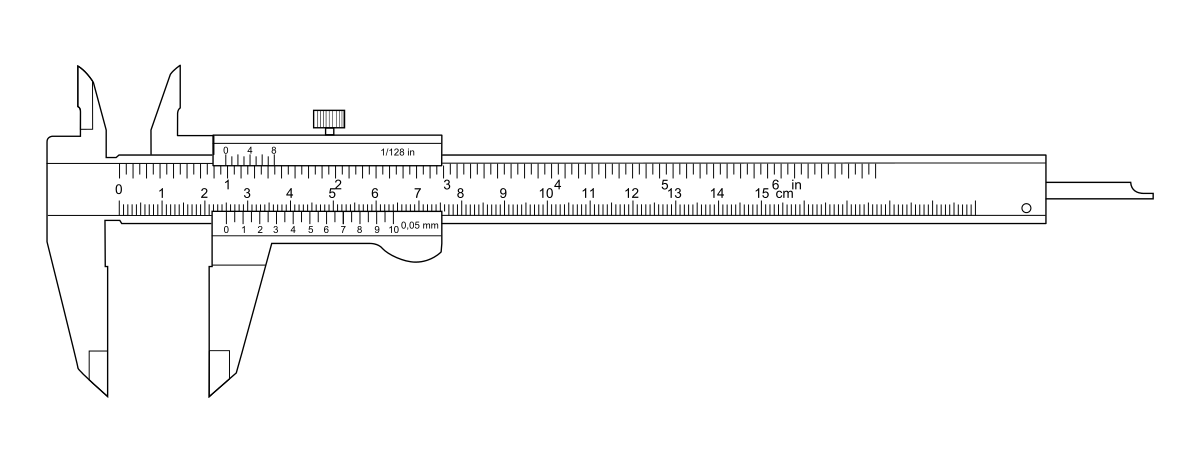
\includegraphics[width=\textwidth]{images/Vernier_Caliper_150mm_lines.svg.png}
    \caption{Шублер}
    \label{fig:caliper}
\end{figure}

Текущото упражнение ще се извърши с помощта на уреди, наречени шублер и микрометър. Принципът на работа и на двата уреда е посредством две скали, едната от които подвижна, а другата - неподвижна.

Илюстрация на шублер е показана на фиг. \ref{fig:caliper}. Този уред може да се използва както за измерване на вътрешната страна на отвори посредством по-близко разположените челюсти, така и за тяхната външна страна посредством по-далечно разположените такива. Шублерът може да измерва и в дълбочина чрез накрайника, издаден вдясно на картината, който е подвижен спрямо основното тяло на инструмента. 

Уредът се употребява по следния начин: на него има разположени две скали, едната от които наричаме подвижна, а другата неподвижна. Подвижната се използва за измерване с по-голяма точност след направено измерване от неподвижната скала. Определянето на по-точната мярка става чрез откриване момента на пресичане на подвижната с неподвижната скала (т.е. тази черта от подвижната скала, която съвпада с коя да е черта от неподвижната). Например, ако взетата мярка от неподвижната скала е 17 mm и се види, че черта от неподвижната скала съвпада с подвижната на четиридесет и третото деление при константа на инструмента 0.02, то измерената стойност се равнява на \begin{math} 17 + 43 \times 0.02 = 17.86 \end{math}. 

\subsection{Микрометър}
\begin{figure}
    \centering
    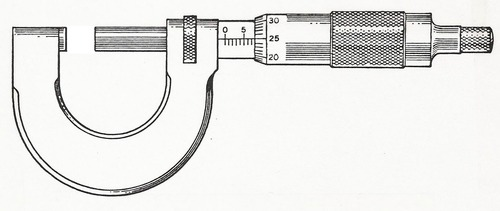
\includegraphics[width=.8\textwidth]{images/micrometers-500x500.jpg}
    \caption{Микрометър}
    \label{fig:micrometer}
\end{figure}

Миркометърът, подобно на шублера, се използва при нужда от измерване на детайли с точността, описана в секция \ref{sec:consts_of_instruments}. Така както шублера, той също се състои от две скали, а именно подвижна и неподвижна, като този път подвижната изпълнява въртеливо движение. 

Подобно на шублера измерването при микрометъра се случва чрез определяне на съвпадението на чертата от подвижната с неподвижната скала и прибавянето на по-малката стойност от подвижната скала към вече определената по-голяма стойност от неподвижната. Препоръчително е подвижната скала да се навива посредством неговата тресчотка ("дръжка"), която предпазва измервания детайл от счупване и/или нараняване в следствие на твърде голяма приложена сила от пренавиване, както и предпазване на самия уред.

\subsection{Константа на инструмента}\label{sec:consts}
Както бе описано в теоритичната част, константата на инструмента, указваща инструменталната грешка при прав нониус, се определя по формулата:
\begin{equation}
k = \frac{a}{n},
\end{equation}\label{eq:meas_consts}
където k - константа на работния инструмент, а - големината на най-малкото скално деление, n - броя на тези най-малки деления. Определянето на констатните на работните шублер и микрометър ще направим по-нататък в ескперименталнта част.

\section{Експериментална част}
Експерименталната част се състои от измерване на малък цилиндричен детайл, диаметърът на който ще бъде измерен чрез шублер (фиг. \ref{fig:caliper}), а височината - чрез микрометър (фиг. \ref{fig:micrometer}).

\subsection{Задача: Определяне на стойностите на константите на използваните в упражнението шублер и микрометър}\label{sec:consts_of_instruments}
Определянето на константите ще направим по формулата, посочена в \ref{sec:consts}. За шублера това е: 

\begin{displaymath}
k = \frac{a}{n} = \frac{1mm}{50} = 0.02 mm,
\end{displaymath}

За микрометъра константата е:

\begin{displaymath}
k = \frac{a}{n} = \frac{0.5mm}{50} = 0.01 mm,
\end{displaymath}

\subsection{Задача: Измерване на линейните размери на тялото}\label{sec:measurements}
Измерването на линейните размери на тялото ще направим чрез няколкократни измервания на един и същи елемент от цилиндъра. Тоест неговите диаметър и височина ще измерим десет пъти. За тази цел създаваме таблица, съдържаща четири колони - номер на измерването; стойността на поредното измерване; отклонението на поредното измерване спрямо средната стойност на този елемент (височина или диаметър); отклонението от предната колона, повдигнато на квадрат и умножено по \begin{math} 10^{-2} \end{math} с цел увеличаване на четимостта на стойностите, използвайки малко по големи стойности. В последния ред на тази таблица изчисляваме средната стойност на съответната величина (формулата е записана в първата колона, а стойността във втората) и сумата на повдигнатия квадрат на отклонението (формулата му е в трета колона, а стойността - в четвърта). Последната стойност, показваща отклонеието на стойността от средната такава на квадрат, също е записана в таблицата с два фактора на десет по-напред (т.е. е умножено по \begin{math}10^{-2}\end{math}. Стойностите са в милиметри (mm).

\begin{table}[h]
\begin{center}
    
\begin{tabular}{|l|l|l|l|}\hline
N   &     d_i, mm     &   d_i - \bar{d}, mm   &   (d_i - \bar{d})^2.10^{-2}, mm^2   \\ \hline
1	&   17.86   &   0.01   &	0.01 \\ \hline
2	&   17.82	&   -0.03	&   0.09 \\ \hline
3	&   17.88	&   0.03	&   0.09 \\ \hline
4	&   17.82	&   -0.03	&   0.09 \\ \hline
5	&   17.84	&   -0.01	&   0.01 \\ \hline
6	&   17.88	&   0.03	&   0.09 \\ \hline
7	&   17.86	&   0.01	&   0.01 \\ \hline
8	&   17.82	&   -0.03	&   0.09 \\ \hline
9	&   17.9	&   0.05	&   0.25 \\ \hline
10	&   17.86	&   0.01	&   0.01 \\ \hline
\specialrule{.1em}{0em}{.2em}
\begin{math} \bar{h} = \frac{\sum_{i=1}^{N}{h_i}}{N} \end{math} &   17.85   &   
\begin{math} \sum_{i=1}^{N}{(h_i - \bar{h})^2} \end{math}       &   0.74    \\ \hline
\end{tabular}

\end{center}
\end{table}



\begin{table}[h]
\begin{center}
    
\begin{tabular}{|l|l|l|l|}\hline
N   &     h_i, mm     &   h_i - \bar{h}, mm   &  (h_i - \bar{h})^2.10^{-2}, mm^2 \\ \hline
1	&   12.04	&   0.01	&   0.01 \\ \hline
2	&   12.03	&   0.00	&   0.00 \\ \hline
3	&   12.04	&   0.01	&   0.01 \\ \hline
4	&   12.01	&   -0.02	&   0.04 \\ \hline
5	&   12.03	&   0.00	&   0.00 \\ \hline
6	&   12.11	&   0.08	&   0.64 \\ \hline
7	&   12.01	&   -0.02	&   0.04 \\ \hline
8	&   12.04	&   0.01	&   0.01 \\ \hline
9	&   12.00	&   -0.03	&   0.09 \\ \hline
10	&   12.00	&   -0.03	&   0.09 \\ \hline
\specialrule{.1em}{0em}{.2em}
\begin{math} \bar{h} = \frac{\sum_{i=1}^{N}{h_i}}{N} \end{math} &   12.03   &   
\begin{math} \sum_{i=1}^{N}{(h_i - \bar{h})^2} \end{math}       &   0.93    \\ \hline
\end{tabular}

\end{center}
\end{table}

\subsection{Задача: Косвено измерване на обема на тялото}

За да открием средната стойност на обема, следваме формулата за обем:
\begin{equation}
    V = \pi \times h \times r^2 = \pi \times \frac{d^2}{4} \times h
\end{equation}

Оттук формулата за средната стойност на обема е:
\begin{equation}
    \bar{V} = \pi \times \frac{\bar{d}^2}{4} \times \bar{h}
\end{equation}

Съгласно формулата по-горе и пресметнатите средни стойности, записани в таблиците на измерените стойности за височина и диаметър получаваме:
\begin{equation}
    \bar{V} = \pi \times \frac{17.85^2}{4} \times 12.03 = 
    \SI{3012.05}{mm^3} = 3012.05 \times 10^{-9} m^3
\end{equation}

За пресмятането на абсолютната грешка с цел записване на отговора във вида \begin{math} V = (\bar{V} \pm \Delta V) \end{math}, използваме формуалта:
\begin{equation}
    \frac{\Delta V}{\bar{V}} = \frac{\Delta \pi}{\pi} + 2\frac{\Delta d}{\bar{d}} + \frac{\Delta h}{\bar{h}}
\end{equation}

Оттук горната формула и от това, че \begin{math} \pi \end{math} е константа, определена с достатъчно голяма точност и нейната грешка не се смята, следва, че абсолютната грешка е \begin{math} \Delta V = (2\frac{\Delta d}{\bar{d}} + \frac{\Delta h}{\bar{h}})\bar{V}\end{math}. За да открием съответните \begin{math}
\Delta d  \end{math} и \begin{math} \Delta h \end{math}, ни е нужно да открием средноквадратичните грешки на диаметъра и височината, тъй като \begin{math} \Delta d = \sqrt{\sigma_d^2 + \Delta_{instr}^2}\end{math}, където \begin{math} \sigma_d \end{math} е средноквадратичната грешка на диаметъра, а \begin{math} \Delta_{instr}^2\end{math} - на инструмента. Аналогично се получава и средноквадратичната грешка на височината: \begin{math} \Delta h = \sqrt{\sigma_h^2 + \Delta_{instr}^2}\end{math}. От стойностите, получени в таблиците в точка \ref{sec:measurements}, пресмятаме стойностите на грешките по-долу. Няма да правим приближение на сметнат корен, а ще приложим директно подкоренните величина във формулите за абсолютна грешка \begin{math}\Delta d \end{math} и \begin{math}\Delta h \end{math}, тъй като там коренът е повдигнат на квадрат.

\begin{equation}
\sigma_d = \sqrt{\frac{\sum(d_i - \bar{d})^2}{N-1}} = \sqrt{\frac{0.74\times10^{-2}}{9}}
\end{equation}

\begin{equation}
\sigma_h = \sqrt{\frac{\sum(h_i - \bar{d})^2}{N-1}} = \sqrt{\frac{0.93\times10^{-2}}{9}} = \sqrt{\frac{0.31\times10^{-2}}{3}}
\end{equation}

Използвайки данните за ининструменталните грешки от \ref{sec:consts_of_instruments} и прилагайки формулите, получаваме:

\begin{equation} 
\Delta d = \sqrt{\sigma_d^2 + \Delta_{instr}^2} = \sqrt{\frac{0.74\times10^{-2}}{9} + 0.02^2} = \frac{\sqrt{110}}{300} \approx 0.0350
\end{equation} 

\begin{equation} 
\Delta h = \sqrt{\sigma_h^2 + \Delta_{instr}^2} = \sqrt{\frac{0.31\times10^{-2}}{3} + 0.01^2} = \frac{\sqrt{102}}{300} \approx 0.0337
\end{equation}

Следователно за абсолютната грешка на обема на тялото получаваме: \begin{equation}
\Delta V = (2\frac{\Delta d}{\bar{d}} + \frac{\Delta h}{\bar{h}})\bar{V} = (2\times \frac{0.0350}{\bar{17.85}} + \frac{0.0337}{\bar{12.03}})\times 3012.05 \approx 20.57
\end{equation} 

Оттук: \begin{math} V = (3012 \pm 21)\times 10^{-9} m^3\end{math}

\end{document}
